\chapter{Objects}
\label{Chp:Objects}

In this chapter, all of the enumerations, literals, data types, and predefined 
opaque objects defined in the GraphBLAS API are presented.  Enumeration literals 
in GraphBLAS are assigned specific values to ensure compatibility between 
different runtime library implementations.  The chapter starts by defining the
enumerations that are used by the {\sf init()} and {\sf wait()} methods.  Then
a number of transparent (i.e., non-opaque) types that are used for interfacing 
with external data are defined.  Sections that follow describe the various
types of opaque objects in GraphBLAS: types (or \emph{domains}), algebraic 
objects, collections and descriptors.  Each of these sections also lists the 
predefined instances of each opaque type that are required by the API.  This chapter
concludes with a section on the definition for {\sf GrB\_Info} enumeration 
that is used as the return type of all methods.

%============================================================================
\section{Enumerations for {\sf init()} and {\sf wait()}}

Table~\ref{Tab:EnumerationModes} lists the enumerations and the corresponding
values used in the {\sf GrB\_init()} method to set the execution mode and in
the {\sf GrB\_wait()} method for completing or materializing opaque objects.

%============================================================================
\section{Indices, index arrays, and scalar arrays}

In order to interface with third-party software (\ie, software other than
an implementation of the GraphBLAS), operations 
such as {\sf GrB\_Matrix\_build} (Section~\ref{Sec:Matrix_build}) and
{\sf GrB\_Matrix\_extractTuples} (Section~\ref{Sec:Matrix_extractTuples}) must specify
how the data should be laid out in  non-opaque data structures.  To 
this end we explicitly define the types for indices and the arrays 
used by these operations.

For indices a {\sf typedef} is used to give a GraphBLAS name to a concrete type. We define it as follows:
\begin{verbatim}
    typedef uint64_t GrB_Index;
\end{verbatim}
The range of valid values for a variable of type {\sf GrB\_Index} is [0, {\sf GrB\_INDEX\_MAX}] 
where the largest index value permissible is defined with a macro, {\sf GrB\_INDEX\_MAX}. For example:
\begin{verbatim}
    #define GrB_INDEX_MAX ((GrB_Index) 0x0fffffffffffffff);
\end{verbatim}
An implementation is required to define and document this value.

An index array is a pointer to a set of {\sf GrB\_Index} values that are 
stored in a contiguous block of memory (\ie, {\sf GrB\_Index*}).
Likewise, a scalar array is a pointer to a contiguous block of memory 
storing a number of scalar values as specified by the user.
Some GraphBLAS operations (\eg, {\sf GrB\_assign})  include an input parameter with the type of an index array. 
This input index array selects a subset of elements from a GraphBLAS vector or matrix object to be used in the operation.
In these cases, the literal {\sf GrB\_ALL} 
can be used in place of the index array input parameter to indicate that all indices 
of the associated GraphBLAS vector or matrix object should be used.
%As with any literal defined in the GraphBLAS, 
An implementation of the GraphBLAS C API has considerable 
freedom in terms of how {\sf GrB\_ALL} is defined.  Since {\sf GrB\_ALL} is used as an argument for an array 
parameter, it must use a type consistent with a pointer. {\sf GrB\_ALL} must also have a non-null
value to distinguish it from the erroneous case of passing a {\sf NULL} pointer as an array.

\begin{table}[b!]
\hrule
\begin{center}
\caption{Enumeration literals and corresponding values input to various GraphBLAS methods.}
\label{Tab:EnumerationModes}

\vspace{1\baselineskip}
(a) {\sf GrB\_Mode} execution modes for the {\sf GrB\_init} method.
\vspace{1\baselineskip}

\begin{tabular}{l|r|p{4in}}
Symbol    & Value & Description \\ \hline
{\sf GrB\_NONBLOCKING}   &  0 & Specifies the nonblocking mode context.\\
{\sf GrB\_BLOCKING}      &  1 & Specifies the blocking mode context. \\
\end{tabular}

\vspace{2\baselineskip}
(b) {\sf GrB\_WaitMode} wait modes for the {\sf GrB\_wait} method.
\vspace{1\baselineskip}

\begin{tabular}{l|r|p{4in}}
Symbol    & Value & Description \\ \hline
{\sf GrB\_COMPLETE}    &  0 & The object is in a state where it can be used in a happens-before relation so that multithreaded programs can be properly synchronized.\\
{\sf GrB\_MATERIALIZE} &  1 & The object is \emph{complete}, and in addition, all computation of the object is finished and any error information is available. \\
\end{tabular}

\end{center}
\hrule
\end{table}

%============================================================================
\section{Types (domains)}
\label{Sec:Domains}

In GraphBLAS, domains correspond to the valid values for types from the
host language (in our case, the C programming language).  GraphBLAS defines
a number of operators that take elements from one or more domains and produce elements of a (possibly) different domain.  GraphBLAS also defines 
three kinds of collections: matrices, vectors and scalars.  For any given 
collection, the elements of the collection belong to a \emph{domain}, which 
is the set of valid values for the elements.  For any variable 
or object $V$ in GraphBLAS we denote as $\mathbf{D}(V)$ the domain of $V$,
that is, the set of possible values that elements of $V$ can take.  

The domains for elements that can be stored in collections and operated on
through GraphBLAS methods are defined by GraphBLAS objects called {\sf GrB\_Type}.
The predefined types and corresponding domains used in the GraphBLAS C API are
shown in Table~\ref{Tab:PredefinedTypes}.  The Boolean type ({\tt bool})
is defined in {\tt stdbool.h}, the integral types ({\tt int8\_t},
{\tt uint8\_t}, {\tt int16\_t}, {\tt uint16\_t}, {\tt int32\_t},
{\tt uint32\_t}, {\tt int64\_t}, {\tt uint64\_t}) are defined in {\tt
stdint.h}, and the floating-point types ({\tt float}, {\tt double}) are
native to the language and platform and in most cases defined by the 
IEEE-754 standard.  UDT stands for user-defined type and is the type returned
for all objects which use a non-predefined type.

\begin{table}
\hrule
\begin{center}
\caption[Predefined {\sf GrB\_Type} values.]{Predefined {\sf GrB\_Type} values, and the corresponding GraphBLAS domain 
suffixes, C type (for scalar parameters), and domains for GraphBLAS.  The domain
suffixes are used in place of $I$, $F$, and $T$ in 
Tables~\ref{Tab:PredefOperators}, \ref{Tab:PredefIndexOperators}, 
\ref{Tab:PredefinedMonoids}, \ref{Tab:PredefinedTrueSemirings}, 
and~\ref{Tab:PredefinedUsefulSemirings}).}
\label{Tab:PredefinedTypes}
\label{Tab:PredefinedDomains}

\vspace{1\baselineskip}
\begin{tabular}{l|l|l|l|l}
{\sf GrB\_Type}   & Enum Value & Suffix       & C type          & Domain \\
\hline
{\sf GrB\_UDT}    & 0          & {\sf UDT}    & -               & -  \\
{\sf GrB\_BOOL}   & 1          & {\sf BOOL}   & {\tt bool}      & $\{ {\tt false}, {\tt true} \}$  \\
{\sf GrB\_INT8}   & 2          & {\sf INT8}   & {\tt int8\_t}   & $\mathbb{Z} \cap [-2^{7},2^{7})$  \\
{\sf GrB\_UINT8}  & 3          & {\sf UINT8}  & {\tt uint8\_t}  & $\mathbb{Z} \cap [0,2{^8})$  \\
{\sf GrB\_INT16}  & 4          & {\sf INT16}  & {\tt int16\_t}  & $\mathbb{Z} \cap [-2^{15},2^{15})$ \\
{\sf GrB\_UINT16} & 5          & {\sf UINT16} & {\tt uint16\_t} & $\mathbb{Z} \cap [0,2^{16})$ \\
{\sf GrB\_INT32}  & 6          & {\sf INT32}  & {\tt int32\_t}  & $\mathbb{Z} \cap [-2^{31},2^{31})$ \\
{\sf GrB\_UINT32} & 7          & {\sf UINT32} & {\tt uint32\_t} & $\mathbb{Z} \cap [0,2^{32})$ \\
{\sf GrB\_INT64}  & 8          & {\sf INT64}  & {\tt int64\_t}  & $\mathbb{Z} \cap [-2^{63},2^{63})$ \\
{\sf GrB\_UINT64} & 9          & {\sf UINT64} & {\tt uint64\_t} & $\mathbb{Z} \cap [0,2^{64})$ \\
{\sf GrB\_FP32}   & 10         & {\sf FP32}   & {\tt float}     & IEEE 754 {\sf binary32}  \\
{\sf GrB\_FP64}   & 11         & {\sf FP64}   & {\tt double}    & IEEE 754 {\sf binary64}  \\

\end{tabular}
\end{center}
\hrule
\end{table}

%============================================================================
\section{Algebraic objects, operators and associated functions}

GraphBLAS operators operate on elements stored in GraphBLAS collections. A 
\emph{binary operator} is a function that maps two input values to one 
output value. A \emph{unary operator} is a function that maps one input value 
to one output value.  Binary operators are defined over two input domains
and produce an output from a (possibly different) third domain. Unary
operators are specified over one input domain and produce an output from a
(possibly different) second domain.

In addition to the operators that operate on stored values, GraphBLAS
also supports \emph{index unary operators} that maps a stored value and 
the indices of its position in the matrix or vector to an output value.
That output value can be used in the index unary operator variants of {\sf apply} (\S~\ref{Sec:Apply}) 
to compute a new stored value, or be used in the {\sf select} operation (\S~\ref{Sec:Select}) to 
determine if the stored input value should be kept or annihilated.

Some GraphBLAS operations require a monoid or semiring.  A monoid contains an associative 
binary operator where the input and output domains are
the same. The monoid also includes an identity value of the operator.
The semiring consists of a binary operator -- referred to as the ``times'' 
operator -- with up to three different domains (two inputs
and one output) and a monoid -- referred to as the ``plus'' operator -- that
is also commutative.  Furthermore, the domain
of the monoid must be the same as the output domain of the ``times'' operator.

The GraphBLAS \emph{algebraic objects} operators, monoids, and semirings
are presented in this section.
These objects can be used as input arguments to various GraphBLAS
operations, as shown in Table~\ref{Tab:OperatorInputType}.
The specific rules for each algebraic object
are explained in the respective sections of those objects.  A summary
of the properties and recipes for building these GraphBLAS algebraic
objects is presented in Table~\ref{Tab:AlgebraicObjects}.

\begin{table}[t]
    \hrule
    \begin{center}
        \caption[Operator input for relevant GraphBLAS operations.]{Operator input for relevant GraphBLAS operations. 
        The semiring add and times are shown if applicable.}
        \label{Tab:OperatorInputType}
        \begin{tabular}{l|l}
        Operation                       & Operator input        \\ \hline
        {\sf mxm, mxv, vxm}             & semiring              \\ \hline
        {\sf eWiseAdd}                  & binary operator       \\
                                        & monoid                \\
                                        & semiring (add)        \\ \hline
        {\sf eWiseMult}                 & binary operator       \\
                                        & monoid                \\
                                        & semiring (times)      \\ \hline
       {\sf reduce} (to vector or {\sf GrB\_Scalar})  & binary operator    \\ 
                                        & monoid                \\ \hline
       {\sf reduce} (to scalar value)   & monoid                \\ \hline
       {\sf apply}                      & unary operator        \\
	                                    & binary operator with scalar \\
                                        & index unary operator  \\ \hline
       {\sf select}                     & index unary operator  \\ \hline
       {\sf kronecker}                  & binary operator       \\
                                        & monoid                \\
                                        & semiring              \\ \hline
       {\sf dup} argument (build methods)     & binary operator \\ \hline
       {\sf accum} argument (various methods) & binary operator \\
       \end{tabular}
    \end{center}
    \hrule
\end{table}

%====================

\begin{table}
    \hrule
    \begin{center}
        \caption[Properties and recipes for building GraphBLAS algebraic objects.]{Properties and recipes for building GraphBLAS algebraic objects: unary operator, binary operator, monoid, and semiring (composed of operations \emph{add} and \emph{times}).}
        \label{Tab:AlgebraicObjects}
        
        \vspace{1\baselineskip}
        (a) Properties of algebraic objects.
        \vspace{1\baselineskip}
        
        \begin{tabular}{l|l|l|l|l}
            Object          & Must be       & Must be        & Identity         & Number \\
                            & commutative   & associative    & must exist       & of domains  \\
            \hline
            Unary operator  & n/a           & n/a            & n/a              & 2  \\
            Binary operator & no            & no             & no               & 3  \\
            Monoid          & no            & yes            & yes              & 1  \\
            Reduction add   & yes           & yes            & yes (see Note 1) & 1  \\
            Semiring add    & yes           & yes            & yes              & 1  \\
            Semiring times  & no            & no             & no               & 3  (see Note 2) \\
        \end{tabular}
        
        \vspace{1\baselineskip}
        (b) Recipes for algebraic objects.
        \vspace{1\baselineskip}
        
        \begin{tabular}{l|l|l}
            Object          & Recipe                                        & Number of domains \\
            \hline
            Unary operator  & Function pointer                              & 2 \\
            Binary operator & Function pointer                              & 3 \\
            Monoid          & Associative binary operator with identity     & 1 \\
            Semiring        & Commutative monoid $+$ binary operator        & 3 \\
        \end{tabular}
        
    \end{center}

        {\footnotesize Note 1: Some high-performance GraphBLAS implementations may require 
        an identity to perform reductions to sparse objects like GraphBLAS vectors 
        and scalars. According to the descriptions of the corresponding GraphBLAS operations, 
        however, this identity is mathematically not necessary.  There are API signatures to
        support both.\newline
        Note 2: The output domain of the semiring times must be same as the domain of the 
        semiring's add monoid. This ensures three domains for a semiring rather than four.}

    \hrule
\end{table}

%====================

A number of predefined operators are specified by the GraphBLAS C API.  They
are presented in tables in their respective subsections below. Each of these 
operators is defined to operate on specific GraphBLAS types and therefore, 
this type is built into the name of the object as a suffix.  These suffixes 
and the corresponding predefined {\sf GrB\_Type} objects that are listed in 
Table~\ref{Tab:PredefinedTypes}.

%----------------------------------------------------------------------------
\subsection{Operators}

A GraphBLAS \emph{unary operator} $F_u = \langle \Dout, \Dinn, f\rangle$
is defined by two domains, $\Dout$ and $\Dinn$, and an operation
$f: \Dinn \rightarrow \Dout$.  For a given GraphBLAS unary operator
$F_u=\langle \Dout, \Dinn, f \rangle$, we define $\bDout(F_u) = \Dout$, 
$\bDinn(F_u) = \Dinn$, and $\mathbf{f}(F_u) = f$.

A GraphBLAS \emph{binary operator} $F_b = \langle \Dout, \Din1, \Din2, 
\odot \rangle$
is defined by three domains, $\Dout$, $\Din1$, $\Din2$, and an operation
$\odot: \Din1 \times \Din2 \rightarrow \Dout$.  For a given GraphBLAS binary operator
$F_b=\langle \Dout, \Din1, \Din2, \odot \rangle$, we define $\bDout(F_b) = \Dout$,
$\bDin1(F_b) = \Din1$, $\bDin2(F_b) = \Din2$, and $\mathbf{\bigodot}(F_b)
= \odot$.  Note that $\odot$ could be used in place of either $\oplus$ or 
$\otimes$ in other methods and operations. 

A GraphBLAS \emph{index unary operator} 
$F_i = \langle \Dout, \Din1, \mathbf{D}({\sf GrB\_Index}), \Din2, f_{i} \rangle$
is defined by three domains, $\Dout$, $\Din1$, $\Din2$, the domain of GraphBLAS 
indices, and an operation
$f_i: \Din1 \times I_{U64}^2 \times \Din2 \rightarrow \Dout$ (where $I_{U64}$ corresponds to the domain of a {\sf GrB\_Index}).  For a given GraphBLAS 
index operator $F_i$, we define $\bDout(F_i) = \Dout$, 
$\bDin1(F_i) = \Din1$, $\bDin2(F_i) = \Din2$, and $\mathbf{f}(F_i) = f_i$.

User-defined operators can be created with calls to {\sf GrB\_UnaryOp\_new}, 
{\sf GrB\_BinaryOp\_new}, and {\sf GrB\_IndexUnaryOp\_new}, respectively.  
See Section~\ref{Sec:AlgebraMethods} for information on these methods.
The GraphBLAS C API predefines a number of these operators.  These are listed 
in Tables~\ref{Tab:PredefOperators} and~\ref{Tab:PredefIndexOperators}.  
Note that most entries in these tables represent a
``family'' of predefined operators for a set of different types represented by
the $T$, $I$, or $F$ in their names.  For example, the multiplicative inverse 
({\sf GrB\_MINV\_$F$}) function is only defined
for floating-point types ($F = $ {\sf FP32} or {\sf FP64}).  The division
({\sf GrB\_DIV\_$T$}) function is defined for all types, but only if $y
\neq 0$ for integral  and floating point types and $y \neq {\tt false}$ for 
the Boolean type.

%====================
\begin{table}
\hspace*{-2.5em}\begin{threeparttable}
\hrule
\caption[Predefined unary and binary operators for GraphBLAS in C.]{Predefined unary and binary operators for GraphBLAS in C.  The $T$ can 
be any suffix from Table~\ref{Tab:PredefinedDomains}, $I$ can be any integer 
suffix from Table~\ref{Tab:PredefinedDomains}, and $F$ can be any floating-point suffix from Table~\ref{Tab:PredefinedDomains}.}
\label{Tab:PredefOperators}
\vspace{1\baselineskip}

\begin{tabular}{l|l|l|ll}
Operator & GraphBLAS             &                                                              & \\
type     & identifier            & Domains                                              & Description \\ \hline
{\sf GrB\_UnaryOp}    & {\sf GrB\_IDENTITY\_$T$} & $T \rightarrow T $     & $f(x) = x$, &identity \\
{\sf GrB\_UnaryOp}    & {\sf GrB\_ABS\_$T$}      & $T \rightarrow T $     & $f(x) = |x|$, &absolute value \\
{\sf GrB\_UnaryOp}    & {\sf GrB\_AINV\_$T$}     & $T \rightarrow T $     & $f(x) = -x$, &additive inverse \\
{\sf GrB\_UnaryOp}    & {\sf GrB\_MINV\_$F$}     & $F \rightarrow F $     & $f(x) = \frac{1}{x}$, &multiplicative inverse \\
{\sf GrB\_UnaryOp}    & {\sf GrB\_LNOT}          & ${\tt bool} \rightarrow {\tt bool}$  & $f(x) =~\neg x$, &logical inverse  \\
{\sf GrB\_UnaryOp}    & {\sf GrB\_BNOT\_$I$}     & $I \rightarrow I$      & $f(x) =~\mbox{\~{}} x$, &bitwise complement \\

&&&\\
{\sf GrB\_BinaryOp}   & {\sf GrB\_LOR}        & ${\tt bool} \times {\tt bool} \rightarrow {\tt bool}$ & $f(x,y) = x \lor y$, & logical OR \\
{\sf GrB\_BinaryOp}   & {\sf GrB\_LAND}       & ${\tt bool} \times {\tt bool} \rightarrow {\tt bool}$ & $f(x,y) = x \land y$, & logical AND \\
{\sf GrB\_BinaryOp}   & {\sf GrB\_LXOR}       & ${\tt bool} \times {\tt bool} \rightarrow {\tt bool}$ & $f(x,y) = x \oplus y$, & logical XOR \\
{\sf GrB\_BinaryOp}   & {\sf GrB\_LXNOR}      & ${\tt bool} \times {\tt bool} \rightarrow {\tt bool}$ & $f(x,y) = \overline{x \oplus y}$, & logical XNOR \\

{\sf GrB\_BinaryOp}   & {\sf GrB\_BOR\_$I$}   & $I \times I \rightarrow I$ & $f(x,y) = x ~|~ y$, & bitwise OR \\
{\sf GrB\_BinaryOp}   & {\sf GrB\_BAND\_$I$}  & $I \times I \rightarrow I$ & $f(x,y) = x ~\&~ y$, & bitwise AND \\
{\sf GrB\_BinaryOp}   & {\sf GrB\_BXOR\_$I$}  & $I \times I \rightarrow I$ & $f(x,y) = x ~\mbox{\^{}}~ y$, & bitwise XOR \\
{\sf GrB\_BinaryOp}   & {\sf GrB\_BXNOR\_$I$} & $I \times I \rightarrow I$ & $f(x,y) = \overline{x ~\mbox{\^{}}~ y}$, & bitwise XNOR \\

{\sf GrB\_BinaryOp}   & {\sf GrB\_EQ\_$T$}    & $T \times T \rightarrow {\tt bool}$  & $f(x,y) = (x == y)$ & equal \\
{\sf GrB\_BinaryOp}   & {\sf GrB\_NE\_$T$}    & $T \times T \rightarrow {\tt bool}$  & $f(x,y) = (x \neq y)$ & not equal \\
{\sf GrB\_BinaryOp}   & {\sf GrB\_GT\_$T$}    & $T \times T \rightarrow {\tt bool}$  & $f(x,y) = (x > y)$ & greater than  \\
{\sf GrB\_BinaryOp}   & {\sf GrB\_LT\_$T$}    & $T \times T \rightarrow {\tt bool}$  & $f(x,y) = (x < y)$ & less than  \\
{\sf GrB\_BinaryOp}   & {\sf GrB\_GE\_$T$}    & $T \times T \rightarrow {\tt bool}$  & $f(x,y) = (x \geq y)$ & greater than or equal \\
{\sf GrB\_BinaryOp}   & {\sf GrB\_LE\_$T$}    & $T \times T \rightarrow {\tt bool}$  & $f(x,y) = (x \leq y)$ & less than or equal \\
{\sf GrB\_BinaryOp}   & {\sf GrB\_ONEB\_$T$}  & $T \times T \rightarrow T$  & $f(x,y) = 1$, & 1 (cast to $T$) \\
{\sf GrB\_BinaryOp}   & {\sf GrB\_FIRST\_$T$} & $T \times T \rightarrow T$  & $f(x,y) = x$, & first argument \\
{\sf GrB\_BinaryOp}   & {\sf GrB\_SECOND\_$T$}& $T \times T \rightarrow T$  & $f(x,y) = y$, & second argument \\
{\sf GrB\_BinaryOp}   & {\sf GrB\_MIN\_$T$}   & $T \times T \rightarrow T$  & $f(x,y) = (x < y)~?~x : y$, & minimum \\
{\sf GrB\_BinaryOp}   & {\sf GrB\_MAX\_$T$}   & $T \times T \rightarrow T$  & $f(x,y) = (x > y)~?~x : y$, & maximum \\
{\sf GrB\_BinaryOp}   & {\sf GrB\_PLUS\_$T$}  & $T \times T \rightarrow T$  & $f(x,y) = x + y$, & addition \\
{\sf GrB\_BinaryOp}   & {\sf GrB\_MINUS\_$T$} & $T \times T \rightarrow T$  & $f(x,y) = x - y$, & subtraction \\
{\sf GrB\_BinaryOp}   & {\sf GrB\_TIMES\_$T$} & $T \times T \rightarrow T$  & $f(x,y) = xy$, & multiplication \\
{\sf GrB\_BinaryOp}   & {\sf GrB\_DIV\_$T$}   & $T \times T \rightarrow T$  & $f(x,y) = \frac{x}{y}$, & division \\
\end{tabular}
\hrule
\comment{
{\sf GrB\_BinaryOp}   & {\sf GrB\_ANY\_$T$}   & $T \times T \rightarrow T$  & $f(x,y) = $ either $x$ or $y$, & either input operand\tnote{1} \\
\begin{tablenotes}
    \item[1] For {\sf GrB\_ANY}, an implementation is free to return either input operand, and is not required to always return the same operand in different invocations.
\end{tablenotes}
}
\end{threeparttable}
\end{table}

%==================
\begin{landscape}

\begin{table}
\hspace{-2.5em}\begin{threeparttable}
\hrule
%\vspace{1\baselineskip}
\caption[Predefined index unary operators for GraphBLAS in C.]{Predefined index unary operators for GraphBLAS in C.  The $T$ can be
any suffix from Table~\ref{Tab:PredefinedDomains}. $I_{U64}$ refers to the 
    unsigned 64-bit, {\sf GrB\_Index}, integer type, $I_{32}$ refers to the signed, 32-bit integer type, and $I_{64}$ refers to signed, 64-bit 
integer type.
The parameters, $u_i$ or $A_{ij}$, are the stored values from the containers 
where the $i$ and $j$ parameters are set to the row and column indices 
corresponding to the location of the stored value. When operating on vectors, 
$j$ will be passed with a zero value. Finally, $s$ is an additional scalar 
value used in the operators.
The expressions in the ``Description'' column are to be treated as mathematical specifications.
    That is, for the index arithmetic functions in the first two groups below, each one of $i$, $j$, and $s$ is interpreted as an integer number in the set $\mathbb{Z}$.
    Functions are evaluated using arithmetic in $\mathbb{Z}$, producing a result value that is also in $\mathbb{Z}$. 
    The result value is converted to the output type according to the rules of the C language. In particular, if the value cannot be represented as a signed 32- or 64-bit integer type, the output is implementation defined.
    Any deviations from this ideal behavior, including limitations on the values of $i$, $j$, and $s$, or possible overflow and underflow conditions, must be defined by the implementation.
    }
\label{Tab:PredefIndexOperators}
%\vspace{1\baselineskip}

    {\small
\begin{tabular}{l|l|cccc|rcll}
Operator type             & GraphBLAS                		& \multicolumn{4}{c|}{Domains ($-$ is don't care)}	& \multicolumn{4}{c}{Description} \\ 
Type                      & Name                     		& $A,u$ & $i$, $j$  	& $s$ 		& result        & &&& \\ \hline
{\sf GrB\_IndexUnaryOp}   & {\sf GrB\_ROWINDEX\_$I_{32/64}$} 	& $-$   & $I_{U64}$	& $I_{32/64}$ 	& $I_{32/64}$ 	& $f(A_{ij},i,j,s)$ & $=$ & $(i + s)$, 		& replace with its row index (+ s) \\
                          &                          		& $-$   & $I_{U64}$ 	& $I_{32/64}$ 	& $I_{32/64}$ 	& $f(u_{i}, i,0,s)$ & $=$ & $(i + s)$  		& \\
{\sf GrB\_IndexUnaryOp}   & {\sf GrB\_COLINDEX\_$I_{32/64}$} 	& $-$   & $I_{U64}$ 	& $I_{32/64}$ 	& $I_{32/64}$ 	& $f(A_{ij},i,j,s)$ & $=$ & $(j + s)$ 		& replace with its column index (+ s) \\
{\sf GrB\_IndexUnaryOp}   & {\sf GrB\_DIAGINDEX\_$I_{32/64}$}	& $-$   & $I_{U64}$ 	& $I_{32/64}$ 	& $I_{32/64}$ 	& $f(A_{ij},i,j,s)$ & $=$ & $(j - i + s)$	& replace with its diagonal index (+ s) \\
\hline

{\sf GrB\_IndexUnaryOp}   & {\sf GrB\_TRIL}    			& $-$ 	& $I_{U64}$ 	& $I_{64}$ 	& {\sf bool} 	& $f(A_{ij},i,j,s)$ & $=$ & $(j \leq i + s)$ 	& triangle on or below diagonal s \\
{\sf GrB\_IndexUnaryOp}   & {\sf GrB\_TRIU}    			& $-$ 	& $I_{U64}$ 	& $I_{64}$ 	& {\sf bool} 	& $f(A_{ij},i,j,s)$ & $=$ & $(j \geq i + s)$ 	& triangle on or above diagonal s \\
{\sf GrB\_IndexUnaryOp}   & {\sf GrB\_DIAG}    			& $-$ 	& $I_{U64}$ 	& $I_{64}$ 	& {\sf bool} 	& $f(A_{ij},i,j,s)$ & $=$ & $(j  ==  i + s)$ 	& diagonal s \\
{\sf GrB\_IndexUnaryOp}   & {\sf GrB\_OFFDIAG} 			& $-$ 	& $I_{U64}$ 	& $I_{64}$ 	& {\sf bool} 	& $f(A_{ij},i,j,s)$ & $=$ & $(j \neq i + s)$ 	& all but diagonal s \\

{\sf GrB\_IndexUnaryOp}   & {\sf GrB\_COLLE}   			& $-$ 	& $I_{U64}$ 	& $I_{64}$ 	& {\sf bool} 	& $f(A_{ij},i,j,s)$ & $=$ & $(j \leq s)$ 	& columns less or equal to s \\
{\sf GrB\_IndexUnaryOp}   & {\sf GrB\_COLGT}   			& $-$ 	& $I_{U64}$ 	& $I_{64}$ 	& {\sf bool} 	& $f(A_{ij},i,j,s)$ & $=$ & $(j >    s)$ 	& columns greater than s \\
{\sf GrB\_IndexUnaryOp}   & {\sf GrB\_ROWLE}   			& $-$ 	& $I_{U64}$ 	& $I_{64}$ 	& {\sf bool} 	& $f(A_{ij},i,j,s)$ & $=$ & $(i \leq s)$, 	& rows less or equal to s \\
                          &                    			& $-$ 	& $I_{U64}$ 	& $I_{64}$ 	& {\sf bool} 	& $f(u_{i}, i,0,s)$ & $=$ & $(i \leq s)$  \\
{\sf GrB\_IndexUnaryOp}   & {\sf GrB\_ROWGT}   			& $-$ 	& $I_{U64}$ 	& $I_{64}$ 	& {\sf bool} 	& $f(A_{ij},i,j,s)$ & $=$ & $(i >    s)$, 	& rows greater than s \\
                          &                    			& $-$ 	& $I_{U64}$ 	& $I_{64}$ 	& {\sf bool} 	& $f(u_{i}, i,0,s)$ & $=$ & $(i >    s)$ \\
\hline
                     
{\sf GrB\_IndexUnaryOp}   & {\sf GrB\_VALUEEQ\_$T$} 		& $T$ 	& $-$ 		& $T$	 	& {\sf bool} 	& $f(A_{ij},i,j,s)$ & $=$ & $(A_{ij} ==   s)$, 	& elements equal to value s \\
                          &                         		& $T$ 	& $-$ 		& $T$ 		& {\sf bool} 	& $f(u_{i}, i,0,s)$ & $=$ & $(u_{i}  ==   s)$ \\
{\sf GrB\_IndexUnaryOp}   & {\sf GrB\_VALUENE\_$T$} 		& $T$ 	& $-$ 		& $T$ 		& {\sf bool} 	& $f(A_{ij},i,j,s)$ & $=$ & $(A_{ij} \neq s)$, 	& elements not equal to value s \\
                          &                         		& $T$ 	& $-$ 		& $T$ 		& {\sf bool} 	& $f(u_{i}, i,0,s)$ & $=$ & $(u_{i}  \neq s)$ \\
{\sf GrB\_IndexUnaryOp}   & {\sf GrB\_VALUELT\_$T$} 		& $T$ 	& $-$ 		& $T$ 		& {\sf bool} 	& $f(A_{ij},i,j,s)$ & $=$ & $(A_{ij} <    s)$, 	& elements less than value s \\
                          &                         		& $T$ 	& $-$ 		& $T$ 		& {\sf bool} 	& $f(u_{i}, i,0,s)$ & $=$ & $(u_{i}  <    s)$ \\
{\sf GrB\_IndexUnaryOp}   & {\sf GrB\_VALUELE\_$T$} 		& $T$ 	& $-$ 		& $T$ 		& {\sf bool} 	& $f(A_{ij},i,j,s)$ & $=$ & $(A_{ij} \leq s)$, 	& elements less or equal to value s \\
                          &                         		& $T$ 	& $-$ 		& $T$ 		& {\sf bool} 	& $f(u_{i}, i,0,s)$ & $=$ & $(u_{i}  \leq s)$ \\
{\sf GrB\_IndexUnaryOp}   & {\sf GrB\_VALUEGT\_$T$} 		& $T$ 	& $-$ 		& $T$ 		& {\sf bool}	& $f(A_{ij},i,j,s)$ & $=$ & $(A_{ij} >    s)$,	& elements greater than value s \\
                          &                         		& $T$ 	& $-$	 	& $T$ 		& {\sf bool} 	& $f(u_{i}, i,0,s)$ & $=$ & $(u_{i}  >    s)$ \\
{\sf GrB\_IndexUnaryOp}   & {\sf GrB\_VALUEGE\_$T$} 		& $T$ 	& $-$ 		& $T$ 		& {\sf bool} 	& $f(A_{ij},i,j,s)$ & $=$ & $(A_{ij} \geq s)$, 	& elements greater or equal to value s \\
                          &                         		& $T$ 	& $-$ 		& $T$ 		& {\sf bool} 	& $f(u_{i}, i,0,s)$ & $=$ & $(u_{i}  \geq s)$ \\
\end{tabular}
    }
\hrule
\end{threeparttable}
\end{table}


\end{landscape}

%-----------------------------------------------------------------------------
%----------------------------------------------------------------------------
\subsection{Monoids}

A GraphBLAS \emph{monoid} $M =
\langle D,\odot,0 \rangle$ is defined by a single domain $D$, an 
\emph{associative}\footnote{\label{Foot:associative}It is expected 
that implementations of the GraphBLAS will utilize floating point arithmetic 
such as that defined in the IEEE-754 standard even though
floating point arithmetic is not strictly associative.} 
operation $\odot: D \times D \rightarrow D$,
and an identity element $0 \in D$.  For a given GraphBLAS monoid $M=\langle
D,\odot,0 \rangle$ we define $\mathbf{D}(M) = D$, $\mathbf{\bigodot}(M) =
\odot$, and $\mathbf{0}(M) = 0$.  A GraphBLAS monoid is equivalent to 
the conventional \emph{monoid} algebraic structure.

Let $F = \langle D,D,D,\odot \rangle$ be an associative GraphBLAS binary operator
with identity element $0 \in D$.  Then $M = \langle F,0 \rangle = \langle
D,\odot,0 \rangle$ is a GraphBLAS monoid. If $\odot$ is commutative,
then $M$ is said to be a \emph{commutative monoid}.
If a monoid $M$ is created using an operator $\odot$ that is
not associative, the outcome of GraphBLAS operations using such a monoid is undefined.

User-defined monoids can be created with calls to {\sf GrB\_Monoid\_new} 
(see Section~\ref{Sec:AlgebraMethods}).
The GraphBLAS C API predefines a number of monoids that are listed 
in Table~\ref{Tab:PredefinedMonoids}.  Predefined monoids are named {\sf
GrB\_\emph{op}\_MONOID\_$T$}, where \emph{op} is the name of the
predefined GraphBLAS operator used as the associative binary operation
of the monoid and $T$ is the domain (type) of the monoid.

%==================

\begin{table}
\centering
\begin{threeparttable}
\hrule
\caption[Predefined monoids for GraphBLAS in C.]{Predefined monoids for GraphBLAS in C. Maximum and minimum values for the 
various integral types are defined in {\tt stdint.h}. Floating-point infinities are 
defined in {\tt math.h}. The $x$ in {\sf UINT}$x$ or {\sf INT}$x$ can be one of 8, 
16, 32, or 64; whereas in {\sf FP}$x$, it can be 32 or 64.}
\label{Tab:PredefinedMonoids}
\vspace{1\baselineskip}

\begin{tabular}{l|l|l|l}
GraphBLAS                   & Domains, $T$           &               & \\
identifier                  & ($T \times T \rightarrow T$) & Identity      & Description \\ \hline
{\sf GrB\_PLUS\_MONOID\_$T$}  & {\sf UINT}$x$  & 0    & addition \\
                            & {\sf INT}$x$   & 0    & \\
                            & {\sf FP}$x$    & 0    & \\
{\sf GrB\_TIMES\_MONOID\_$T$} & {\sf UINT}$x$  & 1    & multiplication \\
                            & {\sf INT}$x$   & 1    & \\
                            & {\sf FP}$x$    & 1    & \\
{\sf GrB\_MIN\_MONOID\_$T$}   & {\sf UINT}$x$  & {\tt UINT$x$\_MAX}  & minimum \\
                            & {\sf INT}$x$   & {\tt INT$x$\_MAX}  & \\
                            & {\sf FP}$x$    & {\tt INFINITY}   & \\
{\sf GrB\_MAX\_MONOID\_$T$}   & {\sf UINT}$x$  & 0                & maximum \\
                            & {\sf INT}$x$   & {\tt INT$x$\_MIN}  & \\
                            & {\sf FP}$x$    & {\tt -INFINITY}   & \\
\comment{
{\sf GrB\_ANY\_MONOID\_$T$}   & $T$    & (implicit)   & either input\tnote{1} \\
                            & & & \\
}
                               & & & \\
{\sf GrB\_LOR\_MONOID\_BOOL}   & {\sf BOOL}  & {\tt false}   & logical OR \\
{\sf GrB\_LAND\_MONOID\_BOOL}  & {\sf BOOL}  & {\tt true}    & logical AND \\
{\sf GrB\_LXOR\_MONOID\_BOOL}  & {\sf BOOL}  & {\tt false}   & logical XOR (not equal) \\
{\sf GrB\_LXNOR\_MONOID\_BOOL} & {\sf BOOL}  & {\tt true}    & logical XNOR (equal) \\
\end{tabular}
\hrule
\comment{
\begin{tablenotes}
    \item[1] For {\sf GrB\_ANY\_MONOID\_T}, an implementation is free to return either input operand, and is not required to always return the same operand in different invocations.  The identity of this monoid is not defined and therefore should not be used in {\sf GrB\_reduce} variants that produce scalars (where an identity could be needed).
\end{tablenotes}
}
\end{threeparttable}
\end{table}

%----------------------------------------------------------------------------
\subsection{Semirings}

A GraphBLAS \emph{semiring}
$S=\langle \Dout, \Din1, \Din2, \oplus, \otimes, 0 \rangle$ is defined by
three domains $\Dout$, $\Din1$, and $\Din2$; an \emph{associative}\footnotemark[\value{footnote}]
and commutative
additive operation $\oplus : \Dout \times \Dout \rightarrow \Dout$; 
a multiplicative operation $\otimes : \Din1 \times \Din2 \rightarrow
\Dout$; and an identity element $0 \in \Dout$.
For a given GraphBLAS semiring $S=\langle \Dout, \Din1,
\Din2, \oplus,\otimes,0 \rangle$ we define $\bDin1(S) = \Din1$,
$\bDin2(S) = \Din2$, $\bDout(S) = \Dout$, $\mathbf{\bigoplus}(S) =
\oplus$, $\mathbf{\bigotimes}(S) = \otimes$, and $\zero(S) = 0$. 

Let $F = \langle \Dout,\Din1,\Din2,\otimes \rangle$ be an operator
and let $A = \langle \Dout,\oplus,0 \rangle$ be a commutative monoid,
then $S= \langle A,F \rangle = \langle \Dout,\Din1,\Din2,\oplus,\otimes,0 \rangle$
is a semiring.

In a GraphBLAS semiring, the multiplicative operator does not have to distribute over the additive operator. 
This is unlike the conventional \emph{semiring} algebraic structure.

Note: There must be one GraphBLAS monoid in every semiring which 
serves as the semiring's additive operator and  
specifies the same domain for its inputs and output parameters. 
If this monoid is not a commutative monoid, the outcome of GraphBLAS
operations using the semiring is undefined.

A UML diagram of the conceptual hierarchy of object classes in GraphBLAS
algebra (binary operators, monoids, and semirings) is shown in 
Figure~\ref{Fig:AlgebraHierarchy}.

\begin{figure}[htb]
    \hrule
    \begin{center}
        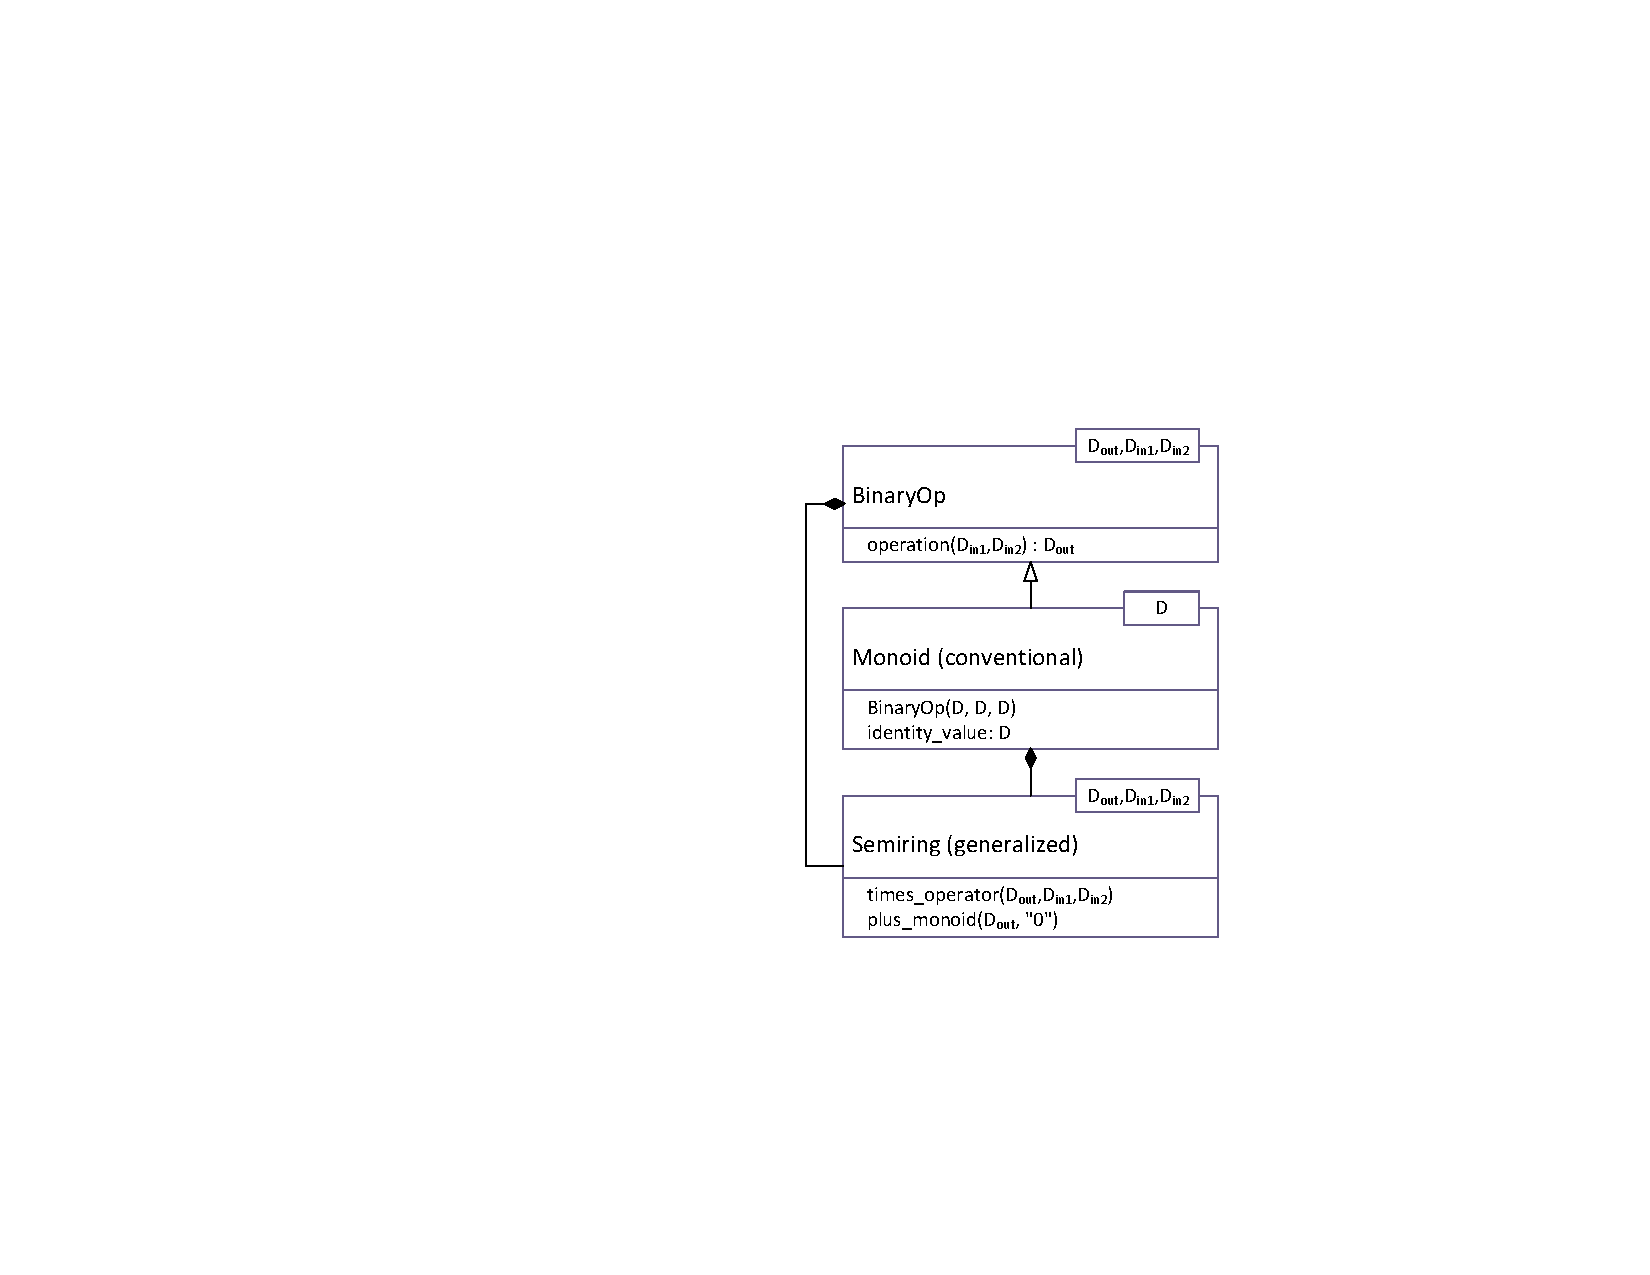
\includegraphics[width=1.0\linewidth,trim=3in 2in 0.5in 2in]{Algebra_Hierarchy_v2_1.pdf}
    \end{center}
    \caption[Hierarchy of algebraic object classes in GraphBLAS.]{Hierarchy of algebraic object classes in GraphBLAS. GraphBLAS 
    semirings consist of a conventional monoid with one domain for the addition 
    function, and a binary operator with three domains for the multiplication function.}
    \label{Fig:AlgebraHierarchy}
    \hrule
\end{figure}

User-defined semirings can be created with calls to {\sf GrB\_Semiring\_new} 
(see Section~\ref{Sec:AlgebraMethods}).
A list of predefined true semirings and convenience
semirings can be found in Tables~\ref{Tab:PredefinedTrueSemirings} and~\ref{Tab:PredefinedUsefulSemirings},
respectively.  Predefined
semirings are named {\sf GrB\_\emph{add}\_\emph{mul}\_SEMIRING\_$T$},
where \emph{add} is the semiring additive operation, \emph{mul} is
the semiring multiplicative operation and $T$ is the domain (type)
of the semiring.

%==================

\begin{table}
\centering
\begin{threeparttable}
\hrule
\caption[Predefined ``true'' semirings for GraphBLAS in C.]{Predefined true semirings 
for GraphBLAS in C where the additive identity is the multiplicative 
annihilator. The $x$ can be one of 8, 16, 32, or 64 in {\sf UINT$x$} or {\sf INT$x$}, 
and can be 32 or 64 in {\sf FP$x$}.}
\label{Tab:PredefinedTrueSemirings}

\hspace*{-1.5em}
\begin{tabular}{l|l|l|l}
                                      & Domains, $T$             & $+$ identity         &                 \\
GraphBLAS identifier              & ($T \times T \rightarrow T$) & $\times$ annihilator & Description     \\ \hline
{\sf GrB\_PLUS\_TIMES\_SEMIRING\_$T$}   & {\sf UINT$x$}            & 0                    & arithmetic semiring \\
                                      & {\sf INT$x$}             & 0                    &                 \\
                                      & {\sf FP$x$}              & 0                    &                 \\
{\sf GrB\_MIN\_PLUS\_SEMIRING\_$T$}     & {\sf UINT$x$}            & {\tt UINT$x$\_MAX}   & min-plus semiring  \\
                                      & {\sf INT$x$}             & {\tt INT$x$\_MAX}    &                 \\
                                      & {\sf FP$x$}              & {\tt INFINITY}       &                 \\
{\sf GrB\_MAX\_PLUS\_SEMIRING\_$T$}     & {\sf INT$x$}             & {\tt INT$x$\_MIN}    & max-plus semiring  \\
                                      & {\sf FP$x$}              & {\tt -INFINITY}      &                 \\
{\sf GrB\_MIN\_TIMES\_SEMIRING\_$T$}    & {\sf UINT$x$}            & {\tt UINT$x$\_MAX}   & min-times semiring \\
{\sf GrB\_MIN\_MAX\_SEMIRING\_$T$}      & {\sf UINT$x$}            & {\tt UINT$x$\_MAX}   & min-max semiring   \\
                                      & {\sf INT$x$}             & {\tt INT$x$\_MAX}    &                 \\
                                      & {\sf FP$x$}              & {\tt INFINITY}       &                 \\
{\sf GrB\_MAX\_MIN\_SEMIRING\_$T$}      & {\sf UINT$x$}            & 0                    & max-min semiring   \\
                                      & {\sf INT$x$}             & {\tt INT$x$\_MIN}    &                 \\
                                      & {\sf FP$x$}              & {\tt -INFINITY}      &                 \\
{\sf GrB\_MAX\_TIMES\_SEMIRING\_$T$}    & {\sf UINT$x$}            & 0                    & max-times semiring \\
{\sf GrB\_PLUS\_MIN\_SEMIRING\_$T$}     & {\sf UINT$x$}            & 0                    & plus-min semiring  \\
                                      &                          &                      &                 \\
{\sf GrB\_LOR\_LAND\_SEMIRING\_BOOL}  & {\sf BOOL}               & {\tt false}          & Logical semiring   \\
{\sf GrB\_LAND\_LOR\_SEMIRING\_BOOL}  & {\sf BOOL}               & {\tt true}           & "and-or" semiring  \\
{\sf GrB\_LXOR\_LAND\_SEMIRING\_BOOL} & {\sf BOOL}               & {\tt false}          & same as {\sf NE\_LAND} \\
{\sf GrB\_LXNOR\_LOR\_SEMIRING\_BOOL} & {\sf BOOL}               & {\tt true}           & same as {\sf EQ\_LOR} \\
\end{tabular}

\hrule
\comment{
\begin{tablenotes}
    \item[1] For {\sf GrB\_ANY\_*\_SEMIRING\_T}, an implementation is free to return any of the results of the application of the "multiply" operator ({\sf FIRST} or {\sf SECOND}), and is not required to always return the same result in different invocations..
\end{tablenotes}
}
\end{threeparttable}
\end{table}

\begin{table}
\centering
\begin{threeparttable}
\hrule
\caption[Other useful predefined semirings for GraphBLAS in C.]{Other useful predefined semirings for GraphBLAS in C that don't have a multiplicative annihilator. 
The $x$ can be one of 8, 16, 32, or 64 in {\sf UINT$x$} or {\sf INT$x$}, 
and can be 32 or 64 in {\sf FP$x$}.}
\label{Tab:PredefinedUsefulSemirings}

\hspace*{-1.5em}
\begin{tabular}{l|l|l|l}
                                    & Domains, $T$             &            &                 \\
GraphBLAS identifier           & ($T \times T \rightarrow T$)  & $+$ identity      & Description             \\ \hline
{\sf GrB\_MAX\_PLUS\_SEMIRING\_$T$}   & {\sf UINT$x$}            & 0                 & max-plus semiring         \\
{\sf GrB\_MIN\_TIMES\_SEMIRING\_$T$}  & {\sf INT$x$}             & {\tt INT$x$\_MAX} & min-times semiring        \\
                                    & {\sf FP$x$}              & {\tt INFINITY}    &                  \\
{\sf GrB\_MAX\_TIMES\_SEMIRING\_$T$}  & {\sf INT$x$}             & {\tt INT$x$\_MIN} & max-times semiring        \\
                                    & {\sf FP$x$}              & {\tt -INFINITY}   &                 \\
{\sf GrB\_PLUS\_MIN\_SEMIRING\_$T$}   & {\sf INT$x$}             & 0                 & plus-min semiring          \\
                                    & {\sf FP$x$}              & 0                 &                 \\ 
{\sf GrB\_MIN\_FIRST\_SEMIRING\_$T$}  & {\sf UINT$x$}            & {\tt UINT$x$\_MAX}& min-select first  semiring     \\
                                    & {\sf INT$x$}             & {\tt INT$x$\_MAX} &                 \\
                                    & {\sf FP$x$}              & {\tt INFINITY}    &                 \\
{\sf GrB\_MIN\_SECOND\_SEMIRING\_$T$} & {\sf UINT$x$}            & {\tt UINT$x$\_MAX}& min-select second semiring     \\
                                    & {\sf INT$x$}             & {\tt INT$x$\_MAX} &                 \\
                                    & {\sf FP$x$}              & {\tt INFINITY}    &                 \\
{\sf GrB\_MAX\_FIRST\_SEMIRING\_$T$}  & {\sf UINT$x$}            & 0                 & max-select first  semiring     \\
                                    & {\sf INT$x$}             & {\tt INT$x$\_MIN} &                 \\
                                    & {\sf FP$x$}              & {\tt -INFINITY}   &                 \\
{\sf GrB\_MAX\_SECOND\_SEMIRING\_$T$} & {\sf UINT$x$}            & 0                 & max-select second semiring     \\
                                    & {\sf INT$x$}             & {\tt INT$x$\_MIN} &                 \\
                                    & {\sf FP$x$}              & {\tt -INFINITY}   &                 \\
\end{tabular}

\hrule
\comment{
\begin{tablenotes}
    \item[1] For {\sf GrB\_ANY\_*\_SEMIRING\_T}, an implementation is free to return any of the results of the application of the "multiply" operator ({\sf FIRST} or {\sf SECOND}), and is not required to always return the same result in different invocations..
\end{tablenotes}
}
\end{threeparttable}
\end{table}

%============================================================================
\section{Collections}

%----------------------------------------------------------------------------
\subsection{Scalars}
\label{Sec:Scalars}

A \emph{GraphBLAS scalar}, $\scalar{s} = \langle D, \{ \sigma \} \rangle$, is defined by
a domain $D$, and a set of zero or one \emph{scalar value}, $\sigma$, where $\sigma \in D$. 
We define $\mathbf{size}(\scalar{s}) = 1$ (constant), and
$\mathbf{L}(\scalar{s}) = \{ \sigma \}$. The set $\mathbf{L}(\scalar{s})$ is
called the \emph{contents} of the GraphBLAS scalar $\scalar{s}$. We also define 
$\mathbf{D}(\scalar{s}) = D$. Finally, $\mathbf{val}(s)$ is a 
reference to the scalar value, $\sigma$, if the GraphBLAS scalar is not empty, and is 
undefined otherwise.

%----------------------------------------------------------------------------
\subsection{Vectors}
\label{Sec:Vectors}

A vector $\vector{v} = \langle D, N, \{ (i,v_i) \} \rangle$ is defined by
a domain $D$, a size $N>0$, and a set of tuples $(i,v_i)$ where $0 \leq
i < N$ and $v_i \in D$. A particular value of $i$ can appear at
most once in $\vector{v}$. We define $\mathbf{size}(\vector{v}) = N$ and
$\mathbf{L}(\vector{v}) = \{ (i,v_i) \}$. The set $\mathbf{L}(\vector{v})$ is
called the \emph{content} of vector $\vector{v}$. We also define the set
$\vector{ind(\vector{v})} = \{ i : (i,v_i) \in \mathbf{L}(\vector{v}) \}$
(called the \emph{structure} of $\vector{v}$), and $\mathbf{D}(\vector{v})
= D$. For a vector $\vector{v}$, $\vector{v}(i)$ is a reference to $v_i$
if $(i,v_i) \in \mathbf{L}(\vector{v})$ and is undefined otherwise.

%----------------------------------------------------------------------------
\subsection{Matrices}
\label{Sec:Matrices}

A matrix $\matrix{A} = \langle D, M, N, \{ (i,j,A_{ij}) \} \rangle$ is
defined by a domain $D$, its number of rows $M>0$, its number of columns
$N>0$, and a set of tuples $(i,j,A_{ij})$ where $0 \leq i < M$, $0 \leq
j < N$, and $A_{ij} \in D$. A particular pair of values $i,j$ can
appear at most once in $\matrix{A}$. We define $\mathbf{ncols}(\matrix{A})
= N$,  $\mathbf{nrows}(\matrix{A}) = M$, and $\mathbf{L}(\matrix{A}) =
\{ (i,j,A_{ij}) \}$.  The set $\mathbf{L}(\matrix{A})$ is called the
\emph{content} of matrix $\matrix{A}$.  We also define the sets
$\vector{indrow(\matrix{A})} = \{ i : \exists (i,j,A_{ij}) \in
\matrix{A} \}$ and $\vector{indcol(\matrix{A})} = \{ j : \exists
(i,j,A_{ij}) \in \matrix{A} \}$.  (These are the sets of nonempty
rows and columns of $\matrix{A}$, respectively.)  The \emph{structure}
of matrix $\matrix{A}$ is the set $\mathbf{ind}(\matrix{A}) = \{ (i,j) :
(i,j,A_{ij}) \in \mathbf{L}(\matrix{A}) \}$, and $\mathbf{D}(\matrix{A}) = D$.
For a matrix $\matrix{A}$, $\matrix{A}(i,j)$ is a reference to $A_{ij}$
if $(i,j,A_{ij}) \in \mathbf{L}(\matrix{A})$ and is undefined otherwise.

If $\matrix{A}$ is a matrix and $0 \leq j < N$, then $\matrix{A}(:,j)
= \langle D, M, \{(i,A_{ij}) : (i,j,A_{ij}) \in \mathbf{L}(\matrix{A})
\} \rangle$ is a vector called the $j$-th \emph{column}
of $\matrix{A}$. Correspondingly, if $\matrix{A}$ is a matrix and
$0 \leq i < M$, then $\matrix{A}(i,:) = \langle D, N, \{(j,A_{ij}) :
(i,j,A_{ij}) \in \mathbf{L}(\matrix{A}) \} \rangle$ is a vector called
the $i$-th \emph{row} of $\matrix{A}$.

Given a matrix $\matrix{A} = \langle D, M, N, \{ (i,j,A_{ij}) \} \rangle$,
its \emph{transpose} is another matrix $\matrix{A}^T = \langle D, N, M, \{
(j,i,A_{ij}) : (i,j,A_{ij}) \in \mathbf{L}(\matrix{A}) \} \rangle$.

%----------------------------------------------------------------------------
\subsubsection{External matrix formats}\label{Sec:GrB_Format}

The specification also supports the export and import of matrices to/from a 
number of commonly used formats, such as COO, CSR, and CSC formats.  When
importing or exporting a matrix to or from a GraphBLAS object using
{\sf GrB\_Matrix\_import} (\S~\ref{Sec:Matrix_import}) or {\sf GrB\_Matrix\_export} (\S~\ref{Sec:Matrix_export}), it is necessary to
specify the data format for the matrix data external to GraphBLAS, which is
being imported from or exported to.  This non-opaque data format is specified
using an argument of enumeration type {\sf GrB\_Format} that is used to 
indicate one of a number of predefined formats.  The predefined values of 
{\sf GrB\_Format} are specified in Table~\ref{Tab:MatrixFormatEnumerationValues}.  
A precise definition of the non-opaque data formats can be found in 
Appendix~\ref{App:Matrix_format_details}.

\begin{table}[bh]
\hrule
\begin{center}
\caption{{\sf GrB\_Format} enumeration literals and corresponding values for 
matrix import and export methods.}
\label{Tab:MatrixFormatEnumerationValues}

\begin{tabular}{l|r|p{3.75in}}
Symbol    & Value & Description \\ \hline
{\sf GrB\_CSR\_FORMAT} & 0 & Specifies the compressed sparse row matrix format.\\
{\sf GrB\_CSC\_FORMAT} & 1 & Specifies the compressed sparse column matrix format.\\
{\sf GrB\_COO\_FORMAT} & 2 & Specifies the sparse coordinate matrix format.\\
% {\sf GrB\_DENSE\_ROW\_FORMAT} & 3 & Specifies the dense row-major matrix format.\\
% {\sf GrB\_DENSE\_COL\_FORMAT} & 4 & Specifies the dense column-major matrix format.\\
\end{tabular}

\end{center}
\hrule
\end{table}


%----------------------------------------------------------------------------
\subsection{Masks}
\label{Sec:Masks}

The GraphBLAS C API defines an opaque object called a \emph{mask}.  The mask
is used to control how computed values are stored in the output from a method. 
The mask is an \emph{internal} opaque object; that is, it is never exposed as a 
variable within an application. 

The mask is formed from input objects to the method that uses 
the mask.  For example, a GraphBLAS method may be called with a matrix as the mask
parameter.   The internal mask object is constructed from the input matrix in one
of two ways.  In the default case, an element of the mask is created for each 
tuple that exists in the matrix for which the value of the tuple cast to Boolean 
evaluates to {\tt true}.  Alternatively, the user can specify {\em structure}-only 
behavior where an element of the mask is created for each tuple that exists in 
the matrix {\em regardless} of the value stored in the input matrix.

The internal mask object can be either a one- or a two-dimensional construct.  
One- and two-dimensional masks, described more formally below, are similar to
vectors and matrices, respectively, except that they have structure
(indices) but no values.  When needed, a value is implied for the elements of a 
mask with an implied value of {\tt true} for elements that exist 
and an implied value of {\tt false} for elements that do not exist (\ie,
the locations of the mask that do not have a stored value imply a value of {\tt false}).
Hence, even though a mask does not contain any values, it can be 
considered to imply values from a Boolean domain.

A one-dimensional mask $\vector{m} = \langle N, \{ i \} \rangle$ is
defined by its number of elements $N>0$, and a set $\mathbf{ind}(\vector{m})$
of indices $\{ i \}$ where $0 \leq i < N$.  A particular value of $i$ can
appear at most once in $\vector{m}$. We define $\mathbf{size}(\vector{m})
= N$. The set $\mathbf{ind}(\vector{m})$ is called the \emph{structure} of mask $\vector{m}$.

A two-dimensional mask $\matrix{M} = \langle M, N, \{ (i,j) \}
\rangle$ is defined by its number of rows $M>0$, its number of
columns $N>0$, and a set $\mathbf{ind}(\matrix{M})$ of tuples $(i,j)$
where $0 \leq i < M$, $0 \leq j < N$.   A particular pair of values
$i,j$ can appear at most once in $\matrix{M}$.  We define
$\mathbf{ncols}(\matrix{M}) = N$, and $\mathbf{nrows}(\matrix{M}) = M$.
We also define the sets $\vector{indrow(\matrix{M})} = \{ i : \exists
(i,j) \in \mathbf{ind}(\matrix{M}) \}$ and $\vector{indcol(\matrix{M})}
= \{ j : \exists (i,j) \in \mathbf{ind}(\matrix{M}) \}$.  These are
the sets of nonempty rows and columns of $\matrix{M}$, respectively.
The set $\mathbf{ind}(\matrix{M})$ is called the \emph{structure} of 
mask $\matrix{M}$.

One common operation on masks is the \emph{complement}.
For a one-dimensional mask $\vector{m}$ this is denoted as
$\neg\vector{m}$. For a two-dimensional mask $\matrix{M}$, this is denoted as
$\neg\matrix{M}$.  The complement of a one-dimensional
mask $\vector{m}$ is defined as $\mathbf{ind}(\neg\vector{m}) = \{i : 0
\leq i < N, i \notin \mathbf{ind}(\vector{m}) \}$.  It is the set of all
possible indices that do not appear in $\vector{m}$.  The 
complement of a two-dimensional mask $\matrix{M}$ is defined as the set
$\mathbf{ind}(\neg\matrix{M}) = \{(i,j)$ : $0 \leq i < M$, $0 \leq j < N$,
$(i,j) \notin \mathbf{ind}(\matrix{M}) \}$.  It is the set of all possible
indices that do not appear in $\matrix{M}$.

%----------------------------------------------------------------------------
%============================================================================

\section{Descriptors}
\label{Sec:Descriptors}

Descriptors are used to modify the behavior of a GraphBLAS method.
When present in the signature of a method, they appear as the last
argument in the method.  Descriptors specify how the other input arguments
corresponding to GraphBLAS collections -- vectors, matrices, and masks
-- should be processed (modified) before the main operation of a method
is performed.  A complete list of
what descriptors are capable of are presented in this section.

The descriptor is a lightweight object.  It is composed of (\emph{field},
\emph{value}) pairs where the \emph{field} selects one of the GraphBLAS objects
from the argument list of a method and the \emph{value} defines the
indicated modification associated with that object.  For example,
a descriptor may specify that a particular input matrix needs to be
transposed or that a mask needs to be complemented (defined
in Section~\ref{Sec:Masks}) before using it in the operation.

For the purpose of constructing descriptors, the arguments of a method
that can be modified are identified by specific field names. The output
parameter (typically the first parameter in a GraphBLAS method) is
indicated by the field name, {\sf GrB\_OUTP}.  The mask is indicated
by the {\sf GrB\_MASK} field name. The input parameters corresponding
to the input vectors and matrices are indicated by {\sf GrB\_INP0}
and {\sf GrB\_INP1} in the order they appear in the signature of the
GraphBLAS method.  The descriptor is an opaque object and hence we do not
define how objects of this type should be implemented.   When referring to
(\emph{field}, \emph{value}) pairs for a descriptor, however, we often use the informal
notation {\sf desc[GrB\_Desc\_Field].GrB\_Desc\_Value} without implying
that a descriptor is to be implemented as an array of structures (in fact,
field values can be used in conjunction with multiple values that are composable).
We summarize all types, field names, and values used with descriptors
in Table~\ref{Tab:DescTypeLiterals}.

\begin{table}
\hrule
\begin{center}
\caption[Descriptor types and literals for fields and values.]{Descriptors are GraphBLAS objects passed as arguments to GraphBLAS 
operations to modify other GraphBLAS objects in the operation's argument list.
A descriptor, {\sf desc}, has one or more (\emph{field}, \emph{value}) pairs indicated 
as  {\sf desc[GrB\_Desc\_Field].GrB\_Desc\_Value}. In this table, we define all types and literals used
with descriptors.}
\label{Tab:DescTypeLiterals}

\vspace{1\baselineskip}
(a) Types used with GraphBLAS descriptors.
\vspace{1\baselineskip}

\begin{tabular}{l|l}
Type                      & Description \\ \hline
{\sf GrB\_Descriptor}     &  Type of a GraphBLAS descriptor object. \\
{\sf GrB\_Desc\_Field}    &  The descriptor field enumeration. \\
{\sf GrB\_Desc\_Value}    &  The descriptor value enumeration. \\
\end{tabular}

\vspace{1\baselineskip}
(b) Descriptor field names of type {\sf GrB\_Desc\_Field} enumeration and corresponding values.
\vspace{1\baselineskip}

\begin{tabular}{l|l|l}
Field Name      & Value  & Description \\ \hline
{\sf GrB\_OUTP} & 0      &  Field name for the output GraphBLAS object. \\
{\sf GrB\_MASK} & 1      &  Field name for the mask GraphBLAS object. \\
{\sf GrB\_INP0} & 2      &  Field name for the first input GraphBLAS object. \\
{\sf GrB\_INP1} & 3      &  Field name for the second input  GraphBLAS object. \\
\end{tabular}

\vspace{1\baselineskip}
(c) Descriptor field values of type {\sf GrB\_Desc\_Value} enumeration and corresponding values.
\vspace{1\baselineskip}

\begin{tabular}{l|l|l}
Value Name           & Value  & Description \\ \hline
(reserved)           & 0      & Unused \\ 
{\sf GrB\_REPLACE}   & 1      & Clear the output object before assigning computed values.\\
{\sf GrB\_COMP}      & 2      & Use the complement of the associated object. When combined \\ 
                     &        & with {\sf GrB\_STRUCTURE}, the complement of the structure of the \\
                     &        & associated object is used without evaluating the values stored. \\
{\sf GrB\_TRAN}      & 3      &  Use the transpose of the associated object.\\
{\sf GrB\_STRUCTURE} & 4      & The write mask is constructed from the structure (pattern of \\
                     &        & stored values) of the associated object. The stored values are \\
                     &        & not examined.\\
\end{tabular}
\end{center}
\hrule
\end{table}

In the definitions of the GraphBLAS methods, we often refer to the
\emph{default behavior} of a method with respect to the action of a
descriptor.   If a descriptor is not provided or if the value associated
with a particular field in a descriptor is not set, the default behavior
of a GraphBLAS method is defined as follows:
\begin{itemize}
\item Input matrices are not transposed.
\item The mask is used, as is, without complementing, and stored values are examined to 
determine whether they evaluate to {\tt true} or {\tt false}.

\item Values of the output object that are not directly modified by the operation are preserved.
\end{itemize}

GraphBLAS specifies all of the valid combinations of (field, value) pairs as 
predefined descriptors. Their identifiers and the corresponding set of 
(field, value) pairs for that identfier are shown in 
Table~\ref{Tab:DefaultDescriptors}.

\newcommand{\grboutp}{{\sf GrB\_OUTP}}
\newcommand{\grbmask}{{\sf GrB\_MASK}}
\newcommand{\grbinp}[1]{{\sf GrB\_INP#1}}
\newcommand{\grbreplace}{{\sf GrB\_REPLACE}}
\newcommand{\grbstructure}{{\sf GrB\_STRUCTURE}}
\newcommand{\grbscmp}{{\sf GrB\_COMP}}

\newcommand{\grbrepl}{{\sf GrB\_REPLACE}}
\newcommand{\grbstrc}{{\sf GrB\_STRUCTURE}}
\newcommand{\grbcomp}{{\sf GrB\_COMP}}
\newcommand{\grbtran}{{\sf GrB\_TRAN}}

\begin{table}[htbp]
    \hrule
    \begin{center}
    \caption[Predefined GraphBLAS descriptors.]{Predefined GraphBLAS descriptors. The list includes
    all possible descriptors, according to the current standard.  Columns list the
    possible fields and entries list the value(s) associated with those fields for
    a given descriptor.}
    \label{Tab:DefaultDescriptors}
~\\
    \begin{small}

        \begin{tabular}{l|llll} 
        Identifier          & {\sf GrB\_OUTP} & {\sf GrB\_MASK} & {\sf GrB\_INP0} & {\sf GrB\_INP1}  \\ \hline
        {\sf GrB\_NULL}     &    --    &    --    &    --    &    --    \\
        {\sf GrB\_DESC\_T1}       &    --    &    --    &    --    & \grbtran \\
        {\sf GrB\_DESC\_T0}       &    --    &    --    & \grbtran &    --    \\
        {\sf GrB\_DESC\_T0T1}     &    --    &    --    & \grbtran & \grbtran \\
        {\sf GrB\_DESC\_C}        &    --    & \grbcomp &    --    &    --    \\
        {\sf GrB\_DESC\_S}        &    --    & \grbstrc &    --    &    --    \\
        {\sf GrB\_DESC\_CT1}      &    --    & \grbcomp &    --    & \grbtran \\
        {\sf GrB\_DESC\_ST1}      &    --    & \grbstrc &    --    & \grbtran \\
        {\sf GrB\_DESC\_CT0}      &    --    & \grbcomp & \grbtran &    --    \\
        {\sf GrB\_DESC\_ST0}      &    --    & \grbstrc & \grbtran &    --    \\
        {\sf GrB\_DESC\_CT0T1}    &    --    & \grbcomp & \grbtran & \grbtran \\
        {\sf GrB\_DESC\_ST0T1}    &    --    & \grbstrc & \grbtran & \grbtran \\
        {\sf GrB\_DESC\_SC}       &    --    & \grbstrc, \grbcomp &    --    &    --    \\
        {\sf GrB\_DESC\_SCT1}     &    --    & \grbstrc, \grbcomp &    --    & \grbtran \\
        {\sf GrB\_DESC\_SCT0}     &    --    & \grbstrc, \grbcomp & \grbtran &    --    \\
        {\sf GrB\_DESC\_SCT0T1}   &    --    & \grbstrc, \grbcomp & \grbtran & \grbtran \\
        {\sf GrB\_DESC\_R}        & \grbrepl &    --    &    --    &    --    \\
        {\sf GrB\_DESC\_RT1}      & \grbrepl &    --    &    --    & \grbtran \\
        {\sf GrB\_DESC\_RT0}      & \grbrepl &    --    & \grbtran &    --    \\
        {\sf GrB\_DESC\_RT0T1}    & \grbrepl &    --    & \grbtran & \grbtran \\
        {\sf GrB\_DESC\_RC}       & \grbrepl & \grbcomp &    --    &    --    \\
        {\sf GrB\_DESC\_RS}       & \grbrepl & \grbstrc &    --    &    --    \\
        {\sf GrB\_DESC\_RCT1}     & \grbrepl & \grbcomp &    --    & \grbtran \\
        {\sf GrB\_DESC\_RST1}     & \grbrepl & \grbstrc &    --    & \grbtran \\
        {\sf GrB\_DESC\_RCT0}     & \grbrepl & \grbcomp & \grbtran &    --    \\
        {\sf GrB\_DESC\_RST0}     & \grbrepl & \grbstrc & \grbtran &    --    \\
        {\sf GrB\_DESC\_RCT0T1}   & \grbrepl & \grbcomp & \grbtran & \grbtran \\
        {\sf GrB\_DESC\_RST0T1}   & \grbrepl & \grbstrc & \grbtran & \grbtran \\
        {\sf GrB\_DESC\_RSC}      & \grbrepl & \grbstrc, \grbcomp &    --    &    --    \\
        {\sf GrB\_DESC\_RSCT1}    & \grbrepl & \grbstrc, \grbcomp &    --    & \grbtran \\
        {\sf GrB\_DESC\_RSCT0}    & \grbrepl & \grbstrc, \grbcomp & \grbtran &    --    \\
        {\sf GrB\_DESC\_RSCT0T1}  & \grbrepl & \grbstrc, \grbcomp & \grbtran & \grbtran \\
        \end{tabular}
    \end{small}

    \end{center}
    \hrule
\end{table}

\section{Fields}
\label{Sec:Fields}

All GraphBLAS objects and implementations contain fields like those in the descriptor, 
which provide information to users and allow setting runtime parameters and hints.
All GraphBLAS objects are required to implement the {\sf GrB\_get}, {\sf GrB\_getPreallocSize},
and {\sf GrB\_set} methods required to query and set these fields.
The library itself also contains several (\emph{field}, \emph{value}) pairs,
which provide defaults to object level fields, and implementation information such as the
version number or implementation name.

The \emph{value}, \emph{field} pairs available for each object are defined in \ref{Tab:Fields},
although implementations may add {\sf GrB\_Field} enum values to extend the behavior of objects
and methods. A field must always be readable, but in many cases may not be writable.
Such read-only fields might contain static, compile-time information such as {\sf GrB\_API\_VER}, 
while others are determined by other operations, such as {\sf GrB\_BLOCKING\_MODE}
which is determined by {\sf GrB\_Init}. 

{\sf GrB\_INVALID\_VALUE} must be returned when attempting to write to fields which are read only.

The {\sf GrB\_NAME} field is a special case regarding writability.
All objects which have a {\sf GrB\_NAME} field default to an empty string.
Collections and {\sf GrB\_Descriptor}s may have their {\sf GrB\_NAME} set at any time.
User-defined algebraic objects and {\sf GrB\_Type}s may only have their {\sf GrB\_NAME}
set once to a globally unique value. Attempting to set this field after it has already
been set will return a {\sf GrB\_ALREADY\_SET} error code. Built-in algebraic objects and
{\sf GrB\_Type}s have names which can be read, but not written to.

The {\sf GrB\_Field} enumeration is defined by the values in Table~\ref{Tab:Fields}, and selected
values are described in Table~\ref{Tab:Field_Desc}.

\subsection{Input Types}
\label{Sec:getset_types}
Allowable types used in {\sf GrB\_get} and {\sf GrB\_set} are {\sf ENUM}, {\sf GrB\_Scalar},
{\sf char*}, and {\sf void*}. Each {\sf GrB\_Field} is associated with exactly one of these
types as defined in Table~\ref{Tab:Fields}. Implementations that add additional {\sf GrB\_Field}s
must document the type associated with each {\sf GrB\_Field}.

\subsubsection{ENUM Handling}
{\sf ENUM} types use standard {\sf INT32} enumerations defined in {\sf C}.
User code should use the enum name rather than the integer value directly when
getting or setting a field value.

\subsubsection{{\sf GrB\_Scalar} Handling}
When calling {\sf GrB\_get}, the user must provide an already initialized {\sf GrB\_Scalar}
object to which the implementation will write a value of the correct element type.
When calling {\sf GrB\_set}, the {\sf GrB\_Scalar}
must not be empty, otherwise a {\sf GrB\_EMPTY\_OBJECT} error is raised.

\subsubsection{String ({\sf char*}) Handling}
When the input to {\sf GrB\_set} is a {\sf char*} the input array is null terminated.
The {\sf GraphBLAS} implementation must copy this array into internal data structures.
Prior to calling {\sf GrB\_get} for strings, {\sf GrB\_getPreallocSize} must be called
with the same arguments, replacing the final {\sf char*} with {\sf int*} to retrieve the
required string buffer size. The user creates a {\sf char} buffer of this size and
pass the pointer to {\sf GrB\_get}. The {\sf GraphBLAS} implementation will write to this
buffer, including a trailing null terminator. The preallocated size returned will include
one extra byte for the null terminator.

\subsubsection{{\sf void*} Handling}
When the input to {\sf GrB\_set} is a {\sf void*}, an extra {\sf int} argument is passed to
indicate the size of the buffer. The {\sf GraphBLAS} implementation must copy this many bytes
from the buffer into internal data structures. Similar to reading strings, prior to calling
{\sf GrB\_get} for {\sf void*}, {\sf GrB\_getPreallocSize} must be called to find the required
buffer size. The user must create a buffer and pass the pointer to {\sf GrB\_get}. The
implementation will write to this buffer.
No standard specification or protocol is required for the contents of {\sf void*}. It is meant
to be a mechanism to allow full freedom for {\sf GraphBLAS} implementations with needs that
cannot be handled using {\sf ENUM}, {\sf GrB\_Scalar}, or {\sf String}s.

\subsection{Hints}
\label{Sec:Hints}
Several fields are {\em hints} (marked {\sf H} in Table~\ref{Tab:Fields}). 
A GraphBLAS implementation is free to ignore a hint and
return {\sf GrB\_SUCCESS}. When {\sf GrB\_get} is called, the provided hint
should be returned by the implementation, even if it chooses to ignore the hint.

\begin{landscape}
\begin{table}
\hrule
\begin{center}
\caption{Field values of type {\sf GrB\_Field} enumeration, corresponding types, and 
the objects which must implement that {\sf GrB\_Field}. {\sf Collection} refers to
{\sf GrB\_Matrix}, {\sf GrB\_Vector}, and {\sf GrB\_Scalar}, {\sf Algebraic} refers to
{\sf Operators}, {\sf Monoids}, and {\sf Semirings}, while {\sf All} refers to all
GraphBLAS objects. Global fields are denoted by {\sf Global}. All fields may be read,
some may be written (denoted by {\sf W}), and some are hints (denoted by {\sf H}) 
which may be ignored by the implementation. For {\sf *} see~\ref{Sec:Fields}}
\label{Tab:Fields}

\begin{tabular}{l|l|l|l|p{1.9in}}
Field Name                             & W \(\mid\) H       & Value & Implementing Objects                  & Type                   \\ \hline
{\sf GrB\_OUTP}                        & W \(\mid\) ---     & 0     & {\sf GrB\_Descriptor}                 & ENUM of {\sf GrB\_Desc\_Value} \\
{\sf GrB\_MASK}                        & W \(\mid\) ---     & 1     & {\sf GrB\_Descriptor}                 & ENUM of {\sf GrB\_Desc\_Value} \\
{\sf GrB\_INP0}                        & W \(\mid\) ---     & 2     & {\sf GrB\_Descriptor}                 & ENUM of {\sf GrB\_Desc\_Value} \\
{\sf GrB\_INP1}                        & W \(\mid\) ---     & 3     & {\sf GrB\_Descriptor}                 & ENUM of {\sf GrB\_Desc\_Value} \\ \hline
{\sf GrB\_NAME}                        & {\sf *}            & 10    & {\sf All}                             & Null terminated char* \\
{\sf GrB\_LIBRARY\_VER\_MAJOR}         & --- \(\mid\) ---   & 11   & {\sf Global}                          & {\sf GrB\_Scalar} (INT32) \\
{\sf GrB\_LIBRARY\_VER\_MINOR}         & --- \(\mid\) ---   & 12   & {\sf Global}                          & {\sf GrB\_Scalar} (INT32) \\
{\sf GrB\_LIBRARY\_VER\_PATCH}         & --- \(\mid\) ---   & 13   & {\sf Global}                          & {\sf GrB\_Scalar} (INT32) \\
{\sf GrB\_API\_VER\_MAJOR}             & --- \(\mid\) ---   & 14   & {\sf Global}                          & {\sf GrB\_Scalar} (INT32) \\
{\sf GrB\_API\_VER\_MINOR}             & --- \(\mid\) ---   & 15   & {\sf Global}                          & {\sf GrB\_Scalar} (INT32) \\
{\sf GrB\_API\_VER\_PATCH}             & --- \(\mid\) ---   & 16   & {\sf Global}                          & {\sf GrB\_Scalar} (INT32) \\
{\sf GrB\_BLOCKING\_MODE}              & --- \(\mid\) ---   & 17   & {\sf Global}                          & ENUM of {\sf GrB\_Mode} \\ \hline
{\sf GrB\_STORAGE\_ORIENTATION\_HINT}  & W \(\mid\) H       & 100   & {\sf Global}, {\sf Collection}        & ENUM of {\sf GrB\_Orientation} \\
{\sf GrB\_STORAGE\_SPARSITY\_HINT}       & W \(\mid\) H       & 101   & {\sf Collection}                      & ENUM of {\sf GrB\_Sparsity} \\
{\sf GrB\_ELTYPE\_CODE}                  & --- \(\mid\) ---  & 102   & {\sf Collection}                      & ENUM of {\sf GrB\_Type} \\ \hline
{\sf GrB\_INPUT1TYPE\_CODE}             & --- \(\mid\) ---   & 103   & {\sf Algebraic}                       & ENUM of {\sf GrB\_Type} \\
{\sf GrB\_INPUT2TYPE\_CODE}             & --- \(\mid\) ---   & 104   & {\sf Algebraic}                       & ENUM of {\sf GrB\_Type} \\
{\sf GrB\_OUTPUTTYPE\_CODE}             & --- \(\mid\) ---   & 105   & {\sf Algebraic}                       & ENUM of {\sf GrB\_Type} \\
{\sf GrB\_ELTYPE\_STRING}                & --- \(\mid\) ---  & 106   & {\sf Collection}                      & Null terminated char* \\
{\sf GrB\_INPUT1TYPE\_STRING}          & --- \(\mid\) ---   & 107   & {\sf Algebraic}                       & Null terminated char* \\
{\sf GrB\_INPUT2TYPE\_STRING}          & --- \(\mid\) ---   & 108   & {\sf Algebraic}                       & Null terminated char* \\
{\sf GrB\_OUTPUTTYPE\_STRING}          & --- \(\mid\) ---   & 109   & {\sf Algebraic}                       & Null terminated char* \\
\hline
\end{tabular}
\end{center}

\end{table}
\end{landscape}

\begin{table}
\hrule
\begin{center}
\caption{Descriptions of select \emph{field}, \emph{value} pairs listed in \ref{Tab:Fields}}
\label{Tab:Field_Desc}

\begin{tabular}{l|p{3.5in}}
Field Name                             & Description \\
\hline
{\sf GrB\_NAME}                        & The name of any GraphBLAS object, \\
                                       & or the name of the library implementation. \\
{\sf GrB\_BLOCKING\_MODE}              & The blocking mode as set by {\sf GrB\_init} \\
{\sf GrB\_STORAGE\_ORIENTATION\_HINT}  & Hint to the library that a collection is best stored in  \\
                                       & a row (lexicographic) or column (colexicographic) major format. \\
{\sf GrB\_STORAGE\_SPARSITY\_HINT}     & Hint to the library that it should use a storage format \\
                                       & appropriate for the expected sparsity of an object. \\
{\sf GrB\_ELTYPE\_(CODE/STRING)}       & The element type of a collection. \\
{\sf GrB\_INPUT1TYPE\_(CODE/STRING)}   & The type of the first argument to an operator. \\
{\sf GrB\_INPUT2TYPE\_(CODE/STRING)}   & The type of the second argument to an operator. \\
{\sf GrB\_OUTPUTTYPE\_(CODE/STRING)}   & The type of the output of an operator. \\
\hline
\end{tabular}
\end{center}

\end{table}

\begin{table}
\hrule
\begin{center}
\caption[Field value enumerations.]{Enumerations not defined elsewhere in the documents and used
when getting or setting fields are defined in the following tables.}
\label{Tab:FieldValueLiterals}

\vspace{1\baselineskip}
(a) Field values of type {\sf GrB\_Orientation}.
\vspace{1\baselineskip}

\begin{tabular}{l|l|l}
Value Name              & Value   & Description \\ \hline
{\sf GrB\_ROWMAJOR }     & 0       & The majority of iteration over the object will be row-wise. \\
{\sf GrB\_COLMAJOR}      & 1       & The majority of iteration over the object will be column-wise. \\
\end{tabular}

\vspace{1\baselineskip}
(b) Field values of type {\sf GrB\_Storage\_Sparsity}.
\vspace{1\baselineskip}

\begin{tabular}{l|l|l}
Field Name              & Value  & Description \\ \hline
{\sf GrB\_DENSE}        & 0      & Most or all of the elements will be populated. \\
{\sf GrB\_SPARSE}       & 1      & A normal amount of sparsity with most rows and columns containing a few values. \\
{\sf GrB\_HYPERSPARSE}  & 2      & Many rows or columns will contain no values, resulting in extreme sparsity. \\
\end{tabular}

\end{center}
\hrule
\end{table}


%============================================================================
\section{{GrB\_Info} return values}

All GraphBLAS methods return a {\sf GrB\_Info} enumeration value. The three
types of return codes (informational, API error, and execution error) and their
corresponding values are listed in Table~\ref{Tab:GrBInfoValues}.

\begin{table}[bh]
\hrule
\begin{center}
\caption{Enumeration literals and corresponding values returned by GraphBLAS methods and operations.}
\label{Tab:GrBInfoValues}

\vspace{1\baselineskip}
(a) Informational return values
\vspace{1\baselineskip}

\begin{tabular}{l|r|p{4.45in}}
Symbol    & Value & Description \\ \hline
{\sf GrB\_SUCCESS}     &  0 & The method/operation completed successfully (blocking mode), or encountered no API errors (non-blocking mode). \\
{\sf GrB\_NO\_VALUE}   &  1 & A location in a matrix or vector is being accessed that has no stored value at the specified location.\\
\end{tabular}

\vspace{1\baselineskip}
(b) API errors
\vspace{1\baselineskip}

\begin{tabular}{l|r|p{3.45in}}
Symbol    & Value & Description \\ \hline
{\sf GrB\_UNINITIALIZED\_OBJECT} & -1 & A GraphBLAS object is passed to a method before {\sf new} was called on it.\\
{\sf GrB\_NULL\_POINTER}         & -2 & A NULL is passed for a pointer parameter. \\
{\sf GrB\_INVALID\_VALUE}        & -3 & Miscellaneous incorrect values. \\
{\sf GrB\_INVALID\_INDEX}        & -4 & Indices passed are larger than dimensions of the matrix or vector being accessed. \\
{\sf GrB\_DOMAIN\_MISMATCH}      & -5 & A mismatch between domains of collections and operations when user-defined domains are in use.\\
{\sf GrB\_DIMENSION\_MISMATCH}~~ & -6 & Operations on matrices and vectors with incompatible dimensions. \\
{\sf GrB\_OUTPUT\_NOT\_EMPTY}    & -7 & An attempt was made to build a matrix or vector using an output object that already contains valid tuples (elements).\\
{\sf GrB\_NOT\_IMPLEMENTED}      & -8 & An attempt was made to call a GraphBLAS method for a combination of input parameters that is not supported by a particular implementation.\\
{\sf GrB\_ALREADY\_SET}          & -9 & An attempt was made to write to a field which may only be written to once.
\end{tabular}

\vspace{1\baselineskip}
(c) Execution errors
\vspace{1\baselineskip}

\begin{tabular}{l|r|p{3.4in}}
Symbol    & Value & Description \\ \hline
{\sf GrB\_PANIC}                  & -101 & Unknown internal error. \\
{\sf GrB\_OUT\_OF\_MEMORY}        & -102 & Not enough memory for operations. \\
{\sf GrB\_INSUFFICIENT\_SPACE}    & -103 & The array provided is not large enough to hold output. \\
{\sf GrB\_INVALID\_OBJECT}        & -104 & One of the opaque GraphBLAS objects (input or output) is in an invalid state caused by a previous execution error. \\
{\sf GrB\_INDEX\_OUT\_OF\_BOUNDS} & -105 & Reference to a vector or matrix element that is outside the defined dimensions of the object. \\
{\sf GrB\_EMPTY\_OBJECT}          & -106 & One of the opaque GraphBLAS objects does not have a stored value. \\
\end{tabular}

\end{center}
\hrule
\end{table}

